\documentclass[12pt]{article}
\usepackage[utf8]{inputenc}
\usepackage[a4paper, margin=2.5cm]{geometry}
\usepackage{setspace}
\usepackage{tocloft}
\usepackage{siunitx}
\usepackage{amsmath}
\usepackage{graphicx}
\usepackage{listings}
\usepackage{tikz}

\begin{document}

\begin{center}

\vspace*{4cm}

\textbf{INSTITUTO ALPHA LUMEN}\\

\vspace{1cm}

FISICA\\

\vspace{1cm}

\textbf{Miniatura de asa de avião - Mecanica dos fluidos}\\

\vspace{2cm}

Alunos: Diego Trigo Araujo e Luis Felipe Nascimento de Freitas\\

\vspace{0.5cm}

Professor responsável\\

\vfill

April 2026

\end{center}

\newpage

\begin{center}
\textbf{\large SUMÁRIO}
\end{center}

\vspace{0.5cm}

\tableofcontents

\newpage

\section{INTRODUÇÃO}

O princípio de Bernoulli afirma que, quanto maior a velocidade de um fluido, menor será sua pressão. Em uma asa, o ar na parte superior se move mais rápido do que na parte inferior, gerando diferença de pressão.

Nesta atividade, será analisada a velocidade do ar acima e abaixo de uma asa de aviao utilizando anemômetros feitos por nós, e explicaremos porque um aviao com mais de $1000Kg$ consegue voar.

\section{OBJETIVOS}

Analisar o comportamento do ar.\\
Medir a velocidade do vento.\\
Verificar a relação entre as velocidades e pressão.\\
Observar o princípio de Bernoulli.

\section{METODOLOGIA EXPERIMENTAL}

\subsection{Reagente e Materiais}

Asa experimental de $20cm$ de largura\\
Through Bore Encoder V1\\
Estrutura de helice com meia esfera oca de raio $5cm$\\
Tunel de $24cm$ de diâmetro\\
Resistores (Pull up)\\
ESP32 Wroom 3D (Microcontrolador para processar os dados) \\
Ventilador


\subsection{Procedimento Experimental}
Para simplificar a representação matemática ao longo do trabalho, adotou-se a seguinte notação:

O índice (1) refere-se às grandezas associadas à superfície inferior da asa;
O índice (2) refere-se às grandezas associadas à superfície superior da asa.

Assim, por exemplo:

\begin{equation}
V_1 \equiv V_{\text{baixo}}, \quad V_2 \equiv V_{\text{cima}} \\
\end{equation}
\begin{equation}
P_1 \equiv P_{\text{baixo}}, \quad P_2 \equiv P_{\text{cima}} \\ 
\end{equation}

onde (V) representa a velocidade do escoamento e (P) a pressão do fluido.
Para observar o princípio de Bernoulli e provar que há diferença entre a velocidade por baixo e por cima da asa, apresentaremos quesitos matematicos e fisicos, e mostraremos no experimento como fisicamente acontece.

Primeiramente, partindo do princípio de Bernoulli, levando em consideração que há uma altura entre o ponto da superfice e qualquer ponto x da curva de cima
Foram posicionados dois anemômetros, um acima e outro abaixo da asa.

\begin{equation}
\textbf{$P_1 + \frac{1}{2}\rho V_1^{2} + \rho g h_1 = P_2 + \frac{1}{2}\rho V_2^{2} + \rho g h_2$} 
\end{equation}

altura da superfície inferior foi definida como referência, de modo que:

\begin{align}
h_1 &= 0 \\
h_2 &= h(x)
\end{align}

onde $h(x)$ representa a altura da superfície superior da asa em função da posição ao longo da corda, a equação de Bernoulli fica:

\begin{equation}
\textbf{$P_1 + \frac{1}{2}\rho V_1^{2} = P_2 + \frac{1}{2}\rho V_2^{2} + \rho g h(x)$} 
\end{equation}

Considerando que o nosso sistema de anemometro mede em $\mathrm{rpm}$, temos que transformar em $\unit{\radian\per\second}$:

\begin{equation}
\textbf{$\omega = f\frac{\pi}{30}$} 
\end{equation}

Agora pegamos a velocidade angular e transformamos na velocidade na ponta da helice, dado o raio como $5 \times 10^-2 \unit{\metre}$ pela expressão:

\begin{align}
v &= \omega r \\
v &= rf\frac{\pi}{30} \\
v &= (5 \times 10^-2) \times f\frac{\pi}{30}
\end{align}
% Substituindo pelos valores conhecidos, consideramos a densidade do ar $\rho \approx 1,225 \unit{\kg\per\cubic\metre}$, a gravidade como $9,81 \unit{\metre\per\second\squared}$ e o a velocidade como o indice 6. a expressão fica:

% \begin{equation}
% \textbf{$P_1 + \frac{1}{2}1,225(5 \cdot 10^-2 \cdot f_1\frac{\pi}{30})^{2} = P_2 + \frac{1}{2} 1,225(5 \cdot 10^-2 \cdot f_2\frac{\pi}{30})^{2} + 1,225 \cdot 9,81 \cdot h_2$} 
% \end{equation}

Para darmos continuidade, teremos que assumir algumas premissas. Como a medição da distribuição das velocidades ao longo da a asa não é viável no arranjo experimental, as velocidades do escoamento nas superfícies inferior e superior foram aproximadas por valores médios representativos, obtidos por dois anemômetros posicionados em pontos fixos dessas superfícies. Dessa forma, o modelo considera velocidades constantes em cada face da asa, permitindo estimar a diferença de pressão e a força de sustentação.
O sistema foi exposto ao vento e as velocidades serão registradas.

Partindo disso, assumiremos que $V_1$ e $ V_2$ são constantes. Considerando a equação de Bernoulli:

\begin{equation}
\textbf{$P_1 + \frac{1}{2}\rho V_{1}^{2} = P_2 + \frac{1}{2}\rho V_2^{2} + \rho g h(x)$} 
\end{equation}

sabemos que $P_1$ é considerado aproximadamente constante ao longo da asa, adotando base na geometria plana da superfície inferior e na hipótese de velocidades constantes. Dito isso, a variação de pressão considerada, será de $P_2$, variando apenas em função de $h(x)$.

A partir da equação de Bernoulli aplicada entre um ponto na superfície inferior e um ponto correspondente na superfície superior da asa, é possível obter uma expressão para a diferença de pressão entre essas regiões. Isolando os termos de pressão, temos:

\begin{equation}
\textbf{$P_1 - P_2 =  \frac{1}{2}\rho (V_{1}^{2} - V_2^{2}) + \rho g h(x)$} 
\end{equation}

Essa expressão mostra que a diferença de pressão entre as superfícies da asa depende de dois fatores: a diferença entre as velocidades do escoamento nas regiões superior e inferior, representada pelo termo dinâmico, e a variação de altura da superfície superior, representada pelo termo gravitacional. No modelo adotado, como $V_1$ e $V_2$ são considerados constantes, a variação espacial da pressão ocorre apenas em função de $h(x)$.

A partir da expressão obtida para a diferença de pressão, pode-se determinar a força de sustentação como a resultante das forças de pressão distribuídas sobre a superfície da asa.

Considerando um elemento infinitesimal de área $dA$, a força diferencial associada à diferença de pressão pode ser escrita como:

\begin{equation}
\textbf{$\vec{F}  = \iint(P_1 - P_2(x))dA$} 
\end{equation}

Considerando que a variação da pressão ocorre apenas ao longo da direção da corda da asa, e que a largura $b$ é constante, a integral pode ser simplificada para:

\begin{equation}
\textbf{$\vec{F}  = b\int_{0}^{c}(P_1 - P_2(x))dA$} 
\end{equation}

Substituindo a expressão obtida anteriormente para a diferença de pressão, temos:

\begin{equation}
\textbf{$F = b\int_{0}^{c} \left[\frac{1}{2}\rho (V_{1}^{2} - V_2^{2}) + \rho g h(x)\right]dA$} 
\end{equation}

De forma mais geral, a força exercida pela pressão sobre um elemento de área da asa pode ser representada vetorialmente por:

\begin{equation}
\textbf{$d\vec{F}  = -p \vec{n} \ dA$}
\end{equation}

em que $p$ representa a pressão local e $\vec{n}$ o vetor normal unitário à superfície. Assim, para a superfície superior, em que a pressão varia ao longo da corda da asa, tem-se:

\begin{equation}
\textbf{$d\vec{F}_2 = -P_2(x) \vec{n} \ dA$}
\end{equation}

Porem, para fins experimentais, iremos considerar $P_1$ e $P_2$ como valores médios constantes ao longo de toda a corda da asa. Dessa forma, a força de sustentação pode ser aproximada para:

\begin{equation}
\textbf{$\vec{F} = \Delta P A$}
\end{equation}

sendo $A$ a area projetada da asa (apenas a parte da superfice), igual a $120cm^2$, pois nem toda a força da pressão na superfície curva aponta pra cima. Destarte, calcularemos apenas componente vertical, que é o que realmente sustenta a asa.

Para que o sistema seja sustentado, a força de sustentação deve ser maior ou igual ao peso total do corpo levantado. Como o peso é dado por $P=mg$, a a condição para elevação do sistema é:

\begin{equation}
\textbf{$F > mg$}
\end{equation}

Assim, a força de sustentação calculada experimentalmente deve ser comparada ao peso total do conjunto para verificar se ela é suficiente para promover sua elevação, sendo sua massa total = $138\text{ g}$, temos que:

\begin{equation}
\textbf{$F > 0,138g$}
\end{equation}

para elevação do sistema.

O sistema experimental, consiste em um escoamento de ar gerado por um ventilador, sobre uma asa de desenhada e impressa em 3D definida por CAD. O escoamento ocorre dentro de um tubo de diametro $24\text{cm}$. Para medir a velocidade do vento, criamos 2 anêmometros constituidos de Through Bore Encoder ligada a uma hélice de meia esfera oca de raio $5cm$. 

O encoder, no seu modo incremental, é um dispositivo utilizados para medir posição angular, velocidade e sentido de rotação em sistemas eletromecânicos. Diferentemente dos encoders absolutos, eles não fornecem a posição diretamente, mas sim uma sequência de pulsos que representam incrementos de movimento. Neste trabalho, a velocidade de rotação (em RPM) é determinada a partir dos sinais de saída de um encoder incremental do tipo \textit{through-bore}, utilizando dois canais defasados, denominados A e B (neste caso, fios azul e amarelo).

A Figura abaixo apresenta uma representação típica dos sinais A e B em quadratura:
\begin{center}
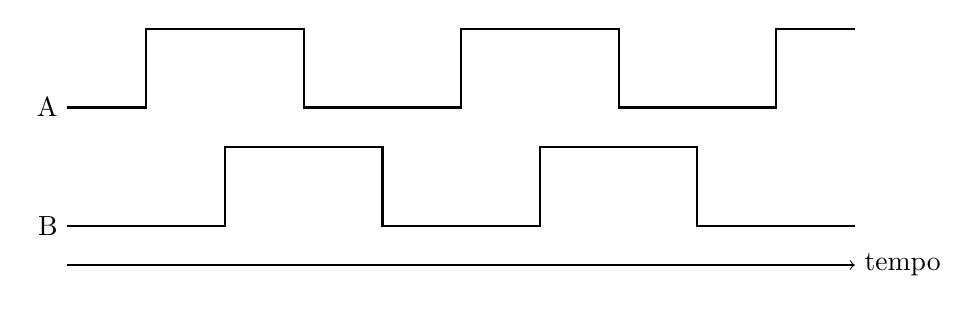
\begin{tikzpicture}[scale=1]
% eixo tempo
\draw[->] (0,0) -- (10,0) node[right] {tempo};
% sinal A
\draw (0,2) node[left] {A};
\draw[thick] (0,2) -- (1,2) -- (1,3) -- (3,3) -- (3,2) -- (5,2) -- (5,3) -- (7,3) -- (7,2) -- (9,2) -- (9,3) -- (10,3);
% sinal B (defasado)
\draw (0,0.5) node[left] {B};
\draw[thick] (0,0.5) -- (2,0.5) -- (2,1.5) -- (4,1.5) -- (4,0.5) -- (6,0.5) -- (6,1.5) -- (8,1.5) -- (8,0.5) -- (10,0.5);
\end{tikzpicture}
\end{center}

Observa-se que o canal B está atrasado em relação ao canal A, caracterizando um dos sentidos de rotação. Caso a ordem dos sinais fosse invertida, o sentido de rotação também seria invertido.
O encoder é caracterizado pelo parâmetro PPR (\textit{Pulses Per Revolution}), que indica o número de pulsos gerados por volta em um único canal. Ao utilizar ambos os canais A e B com detecção de todas as transições (bordas de subida e descida), obtém-se um fator de multiplicação de quatro na resolução do sistema, conhecido como modo x4.

A velocidade de rotação pode ser determinada a partir da contagem do número de transições dos sinais em um intervalo de tempo conhecido. Considerando $N$ como o número de contagens registradas em um intervalo $\Delta t$, a velocidade em rotações por minuto (RPM) é calculada por:
\begin{equation}
RPM = \frac{N \cdot 60}{CPR \cdot \Delta t}
\end{equation}
Substituindo a relação entre CPR e PPR, se tem:
\begin{equation}
RPM = \frac{N \cdot 60}{4 \cdot PPR \cdot \Delta t}
\end{equation}

Além da magnitude da velocidade, o uso dos dois canais permite determinar o sentido de rotação. Quando o canal A antecede o canal B, a rotação ocorre em um sentido; quando o canal B antecede o canal A, a rotação ocorre no sentido oposto. Dessa forma, a contagem pode ser tratada como positiva ou negativa, permitindo a obtenção de velocidade com sinal.
Como exemplo, considere um encoder com $PPR = 1000$. Operando em modo x4, tem-se $CPR = 4000$. Se forem registradas $N = 2000$ contagens em um intervalo de $\Delta t = 0{,}5$ segundos, a velocidade será:
\begin{equation}
RPM = \frac{2000 \cdot 60}{4000 \cdot 0{,}5} = 60
\end{equation}

Para coletar esses dados, utilizamos um \textit{ESP-32 Wroom 32D}, que possui múltiplos pinos GPIO capaz de operar com sinais digitais. Os canais A e B do encoder foram conectados a pinos de entrada digital, como GPIO14 e GPIO27, permitindo a detecção das transições de nível lógico necessárias para a contagem dos pulsos.
Para garantir a integridade dos sinais e evitar leituras instáveis, foram utilizados resistores de \textit{pull-up} de $10\text{k}\Omega$ conectados à tensão de $3{,}3\text{V}$. Essa configuração é especialmente importante quando o encoder possui saída do tipo coletor aberto (open-collector), pois nesses casos o dispositivo apenas força o nível lógico baixo, sendo necessário um resistor externo para definir o nível alto.

No microcontrolador, há um codigo feito em micropython que efetua as operações matematicas de calculo de RPM, e manda esse sinal via \textit{Serial USB-C}, com o comando:


\begin{lstlisting}[language=Python]
print(f"{rpm1:.2f},{rpm2:.2f}")
\end{lstlisting}

Com os dados obtidos do microcontrolador, no meu computador, tratarei os dados de frequencia para diferenca de pressao com a expressão matematica dita anteriormente no índice (12), para força de sustentação, a expressão dita no índice (18), e a velocidade, a expressão dita no índice (10).

\begin{figure}[htbp]
    \centering
    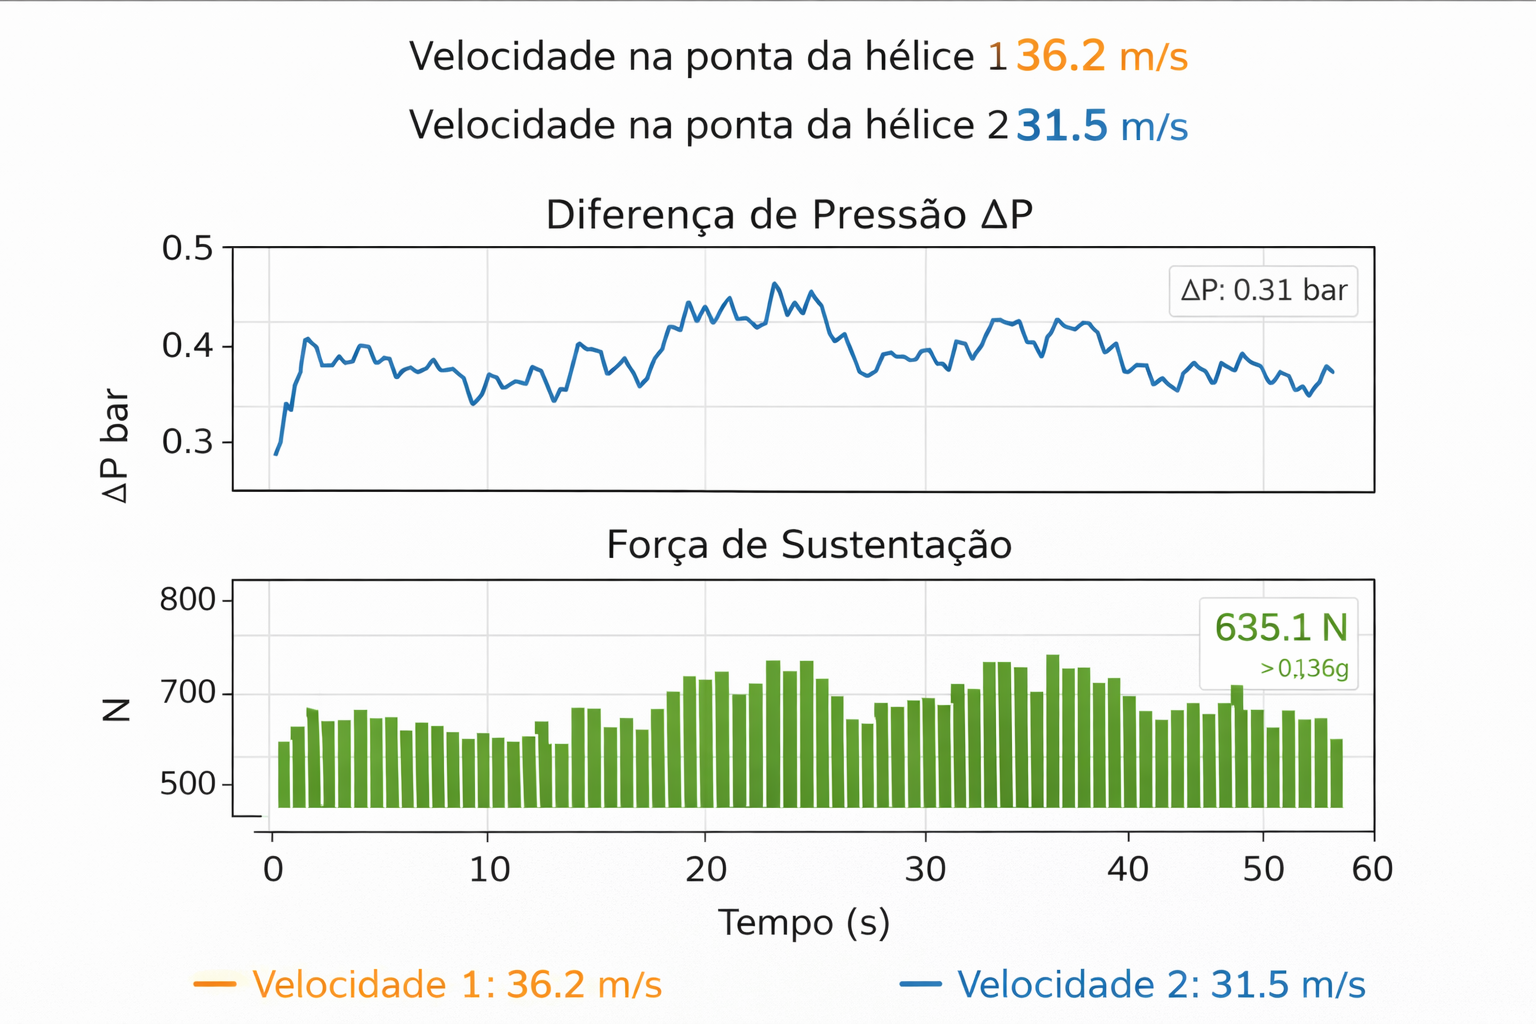
\includegraphics[width=0.9\textwidth]{figures/matplot.png}
    \caption{Grafico no computador (valores ilustrativos)}
    \label{fig:minha_imagem}
\end{figure}


O procedimento do experimento, será primeiramente ligar o circuito dos anemometros, depois ligar o computador, ligar o ventilador e assim, ver os dados sincronizados em tempo real com o computador.

As limitações do projeto é que conseguimos calcular apenas a Pressão e Velocidade média ao longo da asa, tendo imprecisão nos valores obtidos.



\subsection{Tratamento dos Resíduos}

Não houve geração de resíduos.

\section{RESULTADOS E DISCUSSÃO}



\subsection{QUESTIONÁRIO}

1- Como o formato (perfil aerodinâmico) da asa influencia a distribuição de pressão ao seu redor?

2- Qual é o efeito do aumento do ângulo de ataque na sustentação e em que momento ele pode se tornar prejudicial?

3- Por que a sustentação depende do quadrado da velocidade do ar e o que isso implica para o comportamento do avião em diferentes velocidades?

1- O formato da asa, conhecido como perfil aerodinâmico, faz com que o ar escoe mais rapidamente na parte superior e mais lentamente na parte inferior. Isso cria uma diferença de pressão: menor em cima e maior embaixo, gerando sustentação. Perfis mais curvados (cambados) tendem a aumentar essa diferença, enquanto perfis mais simétricos dependem mais do ângulo de ataque para gerar sustentação.

2- O aumento do ângulo de ataque geralmente aumenta a sustentação, pois a asa desvia mais ar para baixo e intensifica a diferença de pressão. No entanto, existe um limite: quando o ângulo fica muito alto, o fluxo de ar se separa da superfície da asa, causando turbulência e perda brusca de sustentação — fenômeno conhecido como estol.

3- A sustentação depende do quadrado da velocidade do ar porque a energia do escoamento (energia cinética) cresce com o quadrado da velocidade. Isso significa que pequenos aumentos na velocidade resultam em aumentos muito maiores na sustentação. Por outro lado, reduções na velocidade diminuem rapidamente a sustentação, o que explica por que aviões precisam manter uma velocidade mínima para continuar voando.


\section{CONCLUSÃO}

Com isso, pode-se perceber que é possível fazer uma miniatura de asa de avião, que demonstra com sucesso as aplicações do princípio de Bernoulli e como isso funcionaria em um avião.  Isso pode ser feito mesmo com materiais baratos, apenas com a engenharia correta. Então assim entendendo como o avião funciona entendendo como o avião funciona, fica mais claro que o voo não depende de “mágica”, mas de um equilíbrio bem controlado entre forças físicas.
A asa, ao interagir com o ar, cria uma diferença de pressão entre a parte superior e inferior, fenômeno frequentemente associado ao Princípio de Bernoulli. No entanto, essa explicação sozinha não conta toda a história. O que realmente sustenta o avião é o fato de que a asa também desvia o fluxo de ar para baixo, gerando uma força de reação para cima, de acordo com as leis do movimento de Isaac Newton.
Ou seja, o voo acontece por uma combinação de diferença de pressão e mudança na direção do fluxo de ar.
Além disso, outros fatores são essenciais. A velocidade do ar influencia diretamente na sustentação: quanto maior a velocidade, maior tende a ser a força gerada. O formato da asa, conhecido como perfil aerodinâmico, também é fundamental, pois define como o ar escoa ao redor dela. Outro ponto importante é o ângulo de ataque, que precisa ser controlado cuidadosamente, já que valores muito altos podem levar à perda de sustentação, conhecida como estol.
No caso da miniatura construída, mesmo utilizando materiais simples, todos esses princípios continuam válidos. Ao medir velocidades e diferenças de pressão, é possível observar na prática como pequenas variações no fluxo de ar resultam em mudanças significativas na sustentação.
Isso demonstra que a engenharia aeronáutica não depende apenas de materiais sofisticados, mas principalmente da aplicação correta dos princípios da física. A partir desse entendimento, é possível avançar para conceitos mais complexos, como controle de voo, otimização de desempenho e estabilidade, aproximando ainda mais o modelo reduzido do comportamento de uma aeronave real.

\end{document}